\chapter{RISC-V}\label{chap:risc-v}
RISC-V is a free and open-source instruction set
architecture (ISA) that was from the start designed to
be modular and extendable. In contrast to many other
ISAs, it can be used for commercial and non-commercial
projects and is freely editable.
This is possible because the ISA is released under the
Berkley Software Distribution (BSD) licenses which do
allow free usage of the ISA and does not require anyone
to release sources for a custom build RISC-V
implementation \cite{risc-v_faq}.
RISC-V is remarkable
because it is designed for a vast range of
applications. The architecture can be tuned for 
microcontrollers, that operate in conditions of limited
resources, as well as for complex multicore systems
with custom extensions \cite{youtube_a_case_for_risc-v}.
The architecture comes with
rich software support including simulators,
compilers (GCC, LLVM, ...), kernels (seL4, Linux, ...),
operating systems (Genode, Debian, ...) and many other
things. More about the software in chapter 
\ref{chap:risc-v,sect:software}.

\section{History}
A predecessor of RISC-V was the academical RISC instruction
set DLX. It was introduced in 1996 by Hennessy and Patterson
and was mainly targeted teaching purposes
\cite{9783540468011}.

In 2010 a new architecture emerged at the University of
Berkeley. Krste Asanović decided to develop and publish
a new architecture that was not only aimed at research
but also for broader applications
\cite{Asanovic_EECS-2014-146}. The project gained
traction and grew over the years.
In 2015 the RISC-V Foundation was founded which
continued to develop the RISC-V ISA. Today the
organization has over 100 members. A small selection
of some platinum members:
\begin{itemize}
    \item Berkeley Architecture Research \footnote{ \url{https://riscv.org/membership/1564/berkeley-architecture-research/}}
    \item Google \footnote{\url{https://riscv.org/membership/999/google/}}
    \item NVIDIA \footnote{\url{https://riscv.org/membership/1437/nvidia/}}
    \item Qualcomm \footnote{\url{https://riscv.org/membership/1585/qualcomm/}}
    \item Samsung \footnote{\url{https://riscv.org/membership/1849/samsung/}}
    \item SiFive \footnote{\url{https://riscv.org/membership/1017/sifive/}}
    \item Western Digital \footnote{\url{https://riscv.org/membership/1020/western-digital/}}
\end{itemize}
\cite{risc-v_members}

\section{Base ISA}
The general architecture of RISC-V is based on a
load-store architecture, which means that "only load
and store instructions access memory and arithmetic 
instructions only operate on CPU registers" 
\cite[p.~18]{risc-v_isa_manual_user_level}.
The minimal set of instructions is called the ISA base.
In the following table \ref{tab:risc-v_isa_base} all current bases can be seen.
\begin{table}[htb]
    \centering
    \begin{tabular}{|l|l|l|l|}
        \hline
        Name & Description & Version & Status \\ \hline
        RV32I & Base Integer Instruction Set, 32-bit & 2.0 & Frozen \\ \hline
        RV32E & Base Integer Instruction Set (embedded), 32-bit, 16 registers
            & 1.9 & Open \\ \hline
        RV64I & Base Integer Instruction Set, 64-Bit & 2.0 & Frozen\\ \hline
        RV128I & Base Integer Instruction Set, 128-Bit & 1.7 & Open\\ 
        \hline
    \end{tabular}
    \caption{RISC-V ISA base \cite[p.~i~\&~v-vi]{risc-v_isa_manual_user_level}}
    \label{tab:risc-v_isa_base}
\end{table}

\subsection{RV32I}
RV32I is the basic instruction set for a 32-bit operating system.
The "I" at the end of the name indicates that this set includes
integer operations. The architecture specifies 32 general-purpose
registers in integer size and a 32-bit user address space.
RV32I is frozen, which means that the design will not change in
the future.

\subsection{RV32E}
RV32E is the embedded implementation of RV32I and an attempt to
"provide an even smaller base core for embedded microcontrollers"
\cite[p.~27]{risc-v_isa_manual_user_level}. The main difference
is that the register count is reduced to 16 registers and not all
extensions can be applied to the design. The following extensions
can be applied:
\begin{itemize}
    \item Atomic instructions (A)
    \item Compressed instructions (C)
    \item Integer multiplication \& division instructions (M)
\end{itemize}
RV32E is not frozen and can be subject to change in the future.

\subsection{RV64I}
The RV64I instruction set builds on RV32I and extends it with
larger registers and a larger user address space (both 64-bit).
Some additional instructions are included to operate on 32-bit
values explicitly. RV64I is already frozen.

\subsection{RV128I}
A higher address space mostly means
a higher amount of addressable memory. As 64 bit can already
address $2^{64}$ bytes = 16 exabytes currently there is no
real need for a 128-bit variant, but in the future, this might
be a useful extension.
The 128-bit variant of the base instruction set extends RV64I like
RV64I did extend RV32I. It is not frozen, as currently,
the expertise for 128-bit real-world applications is missing.

\section{Extensions}
As the base ISAs are kept very minimal (even integer
multiplication is excluded) to enable the implementation
of very minimal cores, standard extensions have been defined to
enable faster hardware implementations.
If an implementation includes certain extensions, the letter is
suffixed behind the base ISA (e.g. RV32IC for a standard 32-bit
base ISA with the compressed instructions extension).
The available standard extensions (their version and their status
can be seen in table \ref{tab:risc-v_isa_extensions}) followed
by the explanations of the extensions.
\begin{table}
    \centering
    \begin{tabular}{|l|l|l|l|}
        \hline
        Name & Description & Version & Status \\ \hline
        A & Atomic instructions & 2.0 & Frozen \\ \hline
        B & Bit manipulation instructions  & 0.36 \cite{github_risc-v_b_extension_release} & Open \\ \hline
        C & Compressed instructions & 2.0 & Frozen \\ \hline
        D & Double-precision floating-point instructions & 2.0 & Frozen\\ \hline
        F & Single-Precision floating-Point instructions & 2.0 & Frozen \\ \hline
        G & General (combination out of I,M,A,F,D) & 2.0 & Frozen \\ \hline
        J & Dynamically translated languages & 0.0 & Open \\ \hline
        L & Decimal floating point instructions & 0.0 & Open \\ \hline
        M & Integer multiplication \& division instructions & 2.0 & Frozen \\ \hline
        N & User-level interrupt instructions & 1.1 & Open \\ \hline
        P & Packed-SIMD instructions & 0.1 & Open \\ \hline
        Q & Quad-precision floating-point instructions & 2.0 & Frozen \\ \hline
        T & Transactional memory instructions & 0.0 & Open \\ \hline
        V & Vector operation instructions & 0.2 & Open \\ \hline
    \end{tabular}
    \caption{RISC-V ISA extensions \cite[p.~i~\&~vi-viii]{risc-v_isa_manual_user_level}}
    \label{tab:risc-v_isa_extensions}
\end{table}
\newline
The following information was taken from the RISC-V Instruction Set Manual
Volume I: User-Level ISA \cite{risc-v_isa_manual_user_level}.

\subsection{Atomic instructions}
The base versions of RISC-V already support the sharing of
memory between multiple hardware threads (harts).
The atomic instructions extension adds additional commands
that help to make handling conditions easier and faster
directly in the hardware. The specification has been frozen.
Two groups of commands are added:
\begin{itemize}
    \item Load-Reserved/Store-Conditional instructions
    \item Atomic memory operations
\end{itemize}

\subsubsection{Load-Reserved/Store-Conditional instructions}
These instructions implement commands to place a reservation on a memory word
to avoid race conditions and undefined states.
These reservations can be broken by other harts, but the original
hart will be notified that his lock is no longer valid, when it
tries to perform a write operation.
This prevents deadlock situations.

\subsubsection{Atomic memory operations}
This instruction group abstracts the steps of performing a
modification of value into one command. They are called
read-modify-write operations. AMOADD, for example, takes in a
source address and an integer value.
The operation will load the value from the source address into
a register, apply an add operation on the value in the register
and the given integer value and writes the result back to the
source address.

\subsection{Bit manipulation instructions}
The B extension, until now, is a placeholder for instructions
that operate on bit size level. These instructions are not finalized
and subject to change.

\subsection{Compressed instructions}
Compressing instructions has two major benefits:
\begin{itemize}
    \item Smaller binary size
    \item Smaller size in cache
\end{itemize}
The smaller size of the binary files especially is beneficial if
the target environment has resource restrictions 
(small embedded devices). The second benefit is important
for high-speed computing applications.
High-speed computers, in general, depend on extensively fast connected
storage. This storage is called cache memory and quite limited in size,
as it is expensive to build.
Compressed instructions make it possible to store more information
in this predefined memory space. This accelerates the execution. In figure 
\ref{fig:kanter_compressed_extension_comparison} a comparison
of the compiled binary file size of the benchmarking program
SPECint2006 can be seen.
\begin{figure}
    \centering
    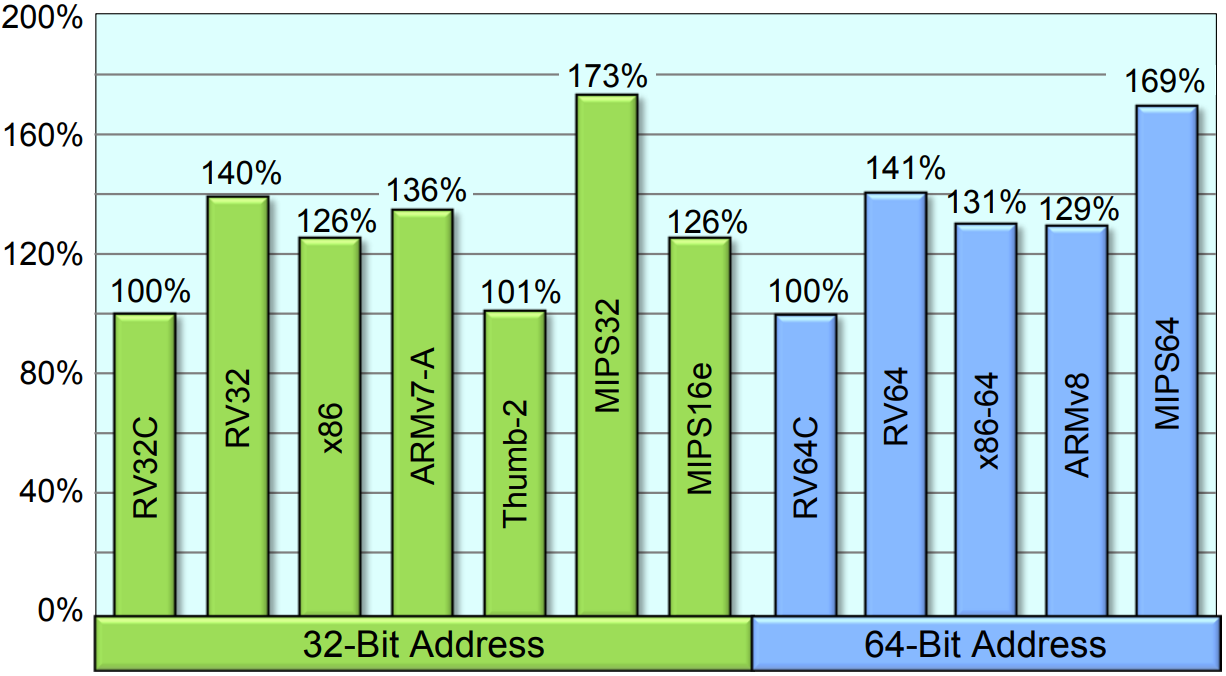
\includegraphics[width=0.5\textwidth]{figures/kanter_compressed_extension_comparison}
    \caption{Comparison of SPECint2006 compilation sizes for different ISAs
        \cite[p.~4]{Kanter_riscv_compressed_figure}, \cite[p.~16]{risc-v_compressed_workshop}}
    \label{fig:kanter_compressed_extension_comparison}
\end{figure}

\subsection{Single-Precision floating-Point instructions}
\textit{Describing this before the Double-precision floating-point instructions as the double-precision extension builds on the single-precision extension.} \newline
This extension implements the classic 32-bit floating-point logic
compliant with the IEEE 754-2008 arithmetic standard \cite{ieee_754-2008}. 
To execute the calculations 32 32-bit registers and one status register
are added.

\subsection{Double-precision floating-point instructions}
This extension builds on the F extension and widens it from a 32-bit to
64-bit size. To hold the larger word sizes the 32 registers
from the F extension are expanded to 64-bit.
The F registers are now capable of holding either 32-bit or
64-bit. The D extension requires the F extension.

\subsection{General}
As a large number of extensions can be overwhelming and
could lead to fragmentation of implementations on the market,
the "general-purpose" ISA extension General was created.
General does not add any additional instructions but
groups the extensions IMAFD together, so a
"general-purpose" RISC-V CPU includes:
\begin{itemize}
    \item Base integer instructions
    \item Integer multiplication \& division instructions
    \item Atomic instructions
    \item Single-Precision floating-Point instructions
    \item Double-precision floating-point instructions
\end{itemize}

\subsection{Dynamically translated languages}
The dynamically translated languages extension is
a placeholder for future standard extensions
to support dynamically translated languages like Java
and Javascript. "These languages can benefit from additional
ISA support for dynamic checks and garbage collection"
\cite[p.~87]{risc-v_isa_manual_user_level}.

\subsection{Decimal floating-point instructions}
The decimal (base-10) floating-point instructions have not been
further specified and the L extension until now is
a placeholder. Still, it is defined that the extension should
be implemented according to the 754-2008 arithmetic standard 
\cite{ieee_754-2008}.

\subsection{Integer multiplication \& division instructions}
These instructions were separated from the base ISAs to enable
low-end implementations that either emulate multiplication and
division instructions or source them out to separate
chipsets. The instructions in these extensions are basic
integer multiplication and division instructions.

\subsection{User-level interrupt instructions}
This extension enables the ISA to forward
interrupts and exceptions directly to user-level
without triggering a context switch.
These instructions could be used for garbage collection
barriers, integer overflow or floating-point traps.

\subsection{Packed-SIMD instructions}
The Single instruction multiple data (SIMD) instructions
allow massive parallel computing on homogeneous data
types (for example: adjusting the brightness of a picture).
This extension does reuse the floating-point registers
and thus does not need additional registers but depends on
the F extension.
The extension is not finished and might be dropped for
a standardized form of the V extension for SIMD operations.

\subsection{Quad-precision floating-point instructions}
The quad-precision floating-point extension widens
the floating-point registers of the previous
floating-point extensions to 128-bit.
The extension requires the RV64I base ISA
and the extensions F and D.

\subsection{Transactional memory instructions}
\label{chap:transactional_memory_instructions}
This instructions are a placeholder and thus not frozen.
Transactional memory is supposed to make working
with multiple threads easier, as syncing memory
between threads can be a big challenge
\cite{gnu_gcc_transactional_memory}.\newline
"Despite much research over the last twenty years
and initial commercial implementations, there
is still much debate on the best way to support 
atomic operations involving multiple addresses.
Our current thoughts are to include a small
limited-capacity transactional memory buffer
along the lines of the original transactional
memory proposals"
\cite[p.~89]{risc-v_isa_manual_user_level}.

\subsection{Vector operation instructions}
This extension is in an early stage and represents
a proposal for a RISC-V vector extension.
"The vector extension supports a configurable vector 
unit, to trade off the number of architectural vector
registers and supported element widths against
available maximum vector length"
\cite[p.~93]{risc-v_isa_manual_user_level}.
This enables different sizes of implementations
to handle the same binary code.
The minimal implementations can be built small,
as they can split up the commands into multiple
smaller commands internally. Larger implementations
can utilize parallelism to speed up the execution.

\subsection{Future extensions}
At the Santa Cara Convention Center on the 2018-12-04
Krste Asanovic listed some future extensions that
will come to the RISC-V ISA:
\cite[p.~14]{risc-v_state_of_the_union_dec_2018}.
\begin{itemize}
    \item Fast interrupts (CLIC) - stable, ratifiable in 2019?
    \item V extension (Vectors) - getting stable, ratifiable in 2019?
    \item Hypervisor extension - stable, ratifiable in 2019?
    \item Crypto (builds on vectors) - builds on vectors
    \item TEE (trusted execution environments) - refocused
    \item B extension (Bit Manipulation) - recently restarted
    \item J extension (dynamic translation support) - ongoing discussion
    \item P extension (DSP extensions) - recently started
    \item Sv128 (Large secure address space) - recently started
\end{itemize}
As the one-character naming scheme limits the amount of
possible names for future extensions, multiple
characters for an abbreviation of an extension
are now allowed.

\section{Software} \label{chap:risc-v,sect:software}
The amount of software that was built or extended
for RISC-V has grown tremendously.
In the following section, some projects that support
RISC-V will be presented. This list is far from
containing all RISC-V capable software, as
a complete list with full descriptions would be
out of scope for this bachelor thesis.
A larger list can be found here:
\footnote{\url{https://riscv.org/software-status/}}.

\subsection{Simulators}
To develop and test an architecture, simulators are
an important quick start option.
For RISC-V already exist eleven simulators with
varying functionality \cite{risc-v_software_status}.
Some of these are described in the following.

\subsubsection{QEMU}
One prominent emulator is the open source machine
emulator quick emulator (QEMU) which also powers
large virtualization solution like Proxmox
\cite{proxmox_qemu_wiki}.
QEMU can be obtained from the project GitHub site
and built on most Linux machines \cite{github_riscv_qemu}.
QEMU is a functional emulator for the RISC-V ISA
which means it directly translates RISC-V instructions
to the host CPU instructions \cite{sifive_risc-v_emulators}.
The downside of this approach is that the emulation does
not provide an instruction-by-instruction trace.
This would normally help to debug the code.

\subsubsection{Spike}
A (outside of the RISC-V world)
less know emulator is the Spike emulator.
The Spike emulator is considered the "golden reference"
simulator \cite{sifive_risc-v_emulators} for the
RISC-V ISA. It is working on a trace accurate
basis, which means the emulator can give the developer
hints if debugging is needed. Additionally, it is built
to be easily editable.
The speed compared
to QEMU is about ten times slower 
(QEMU: 100 million to >1 billion instructions per second
versus Spike: 10 to 100 million instructions per second
\cite{sifive_risc-v_emulators}).

\subsubsection{FireSim}
Another approach is lead by FireSim.
FireSim is an "FPGA-Accelerated Cycle-Exact Scale-Out
System Simulation in the Public Cloud"
\cite{firesim_fpga_accelerated} paper title.
FireSim uses FPGAs in the Amazon cloud to
simulate one or multiple RISC-V implementations
like Berkeley Out-of-Order Machine (BOOM), Rocket-Chip
and more.
As FPGAs often run below the clock rates of the target
tape-out environment, FireSim supports delaying I/O
operations to simulate correct hardware behavior.
\begin{figure}
    \centering
    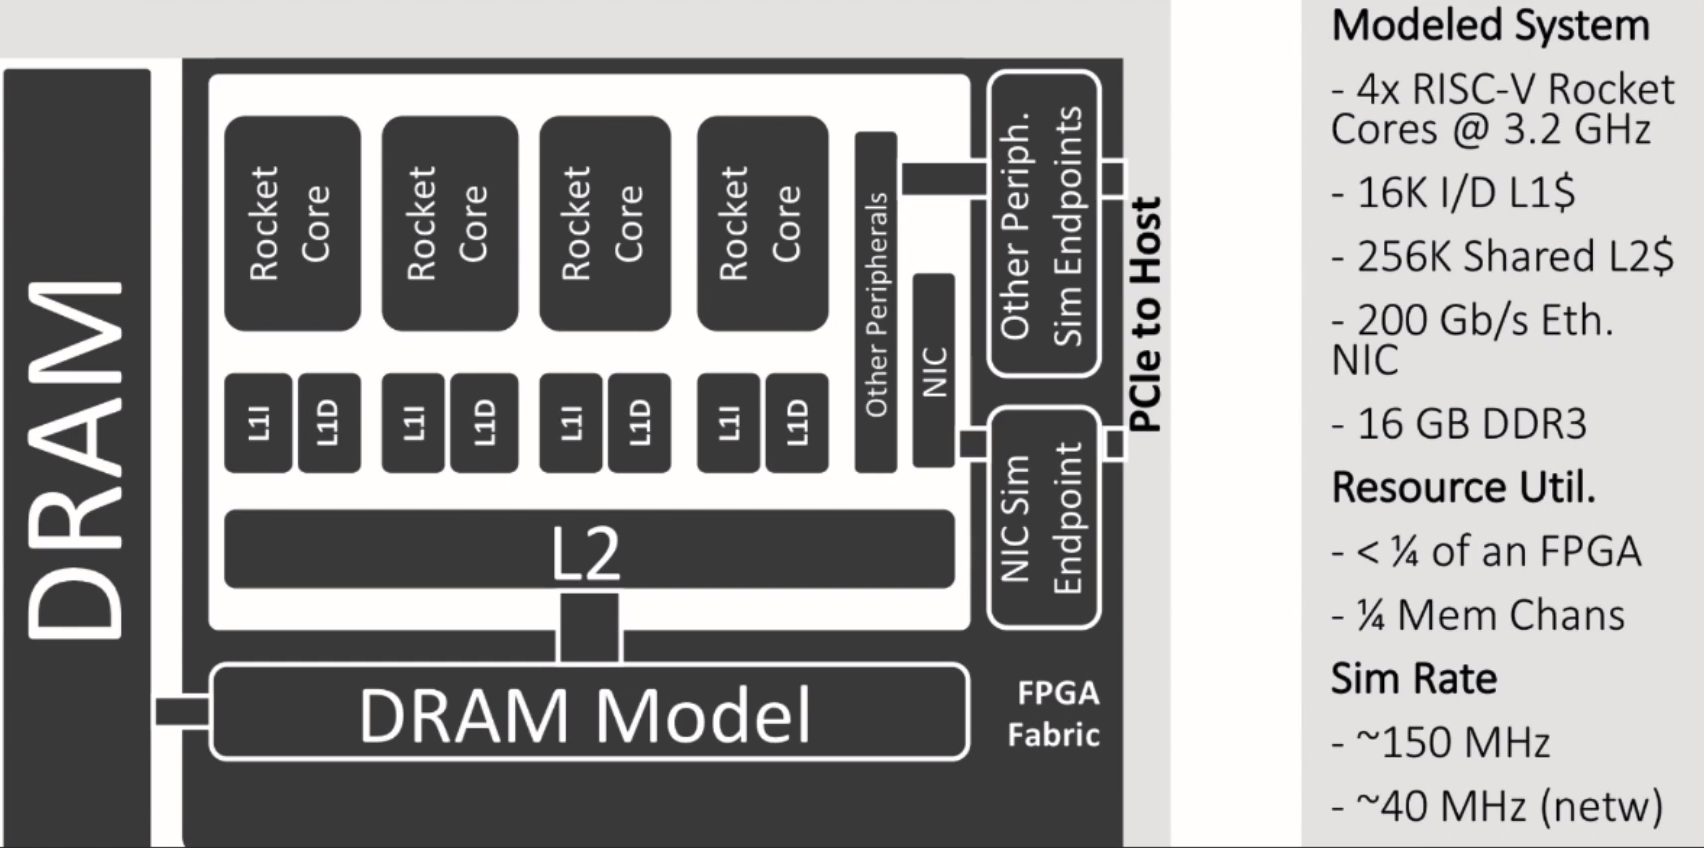
\includegraphics[width=0.8\textwidth]{figures/firesim_riscv_on_fpga}
    \caption{Schematic of a RISC-V processor simulated in FireSim
        \cite[min.~9:00]{chisel_community_firesim}}
    \label{fig:firesim_riscv_on_fpga}
\end{figure}
A schematic of a simulated RISC-V quadcore can be
seen in figure \ref{fig:firesim_riscv_on_fpga}.
The core simulation runs at 150 MHz with a 40 MHz
network simulation. The processor sees itself as running
at 3.2 GHz. The RAM access and the
network access are scaled down to the speed of the
simulation. The observed time of the processor
runs $3200 MHz/150 MHz = 21,\overline{3}$ times slower
than real time.
This project enables developers to test their
implementation on costly FPGA equipment for
a low lease price. Small instances with one 
Xilinx UltraScale+ FPGA \cite{xilinx_amazon_ultrascale}
start at an "On-Demand" price of 1.65 USD
\cite{amazon_fpga_instances}.
In the presentation at the Chisel Community Conference
a whole datacenter simulation was shown that runs 4096
RISC-V cores grouped on 1024 "servers" on 256 FPGAs
\cite[min.~12:08]{chisel_community_firesim}.
FireSim is an open-source project.

\subsubsection{Web-Emulators}
With the advancements of JavaScript over the last years
it is even possible to run a RISC-V emulation in the
web browser. The projects riscv-angel \cite{github_riscv-angel}
can boot a Linux kernel with Busybox
installed on an RV64IMA implementation
directly in the browser in about 3 seconds.
The system is very minimal but still functional.
Another project named JSLinux \cite{bellard_jslinux}
can even boot Fedora with 3D output,
although the system takes a very
long time to boot up. The low performance might
stem from the fact that the developer implemented
an RV128IMAFDQC core. A 128-bit architecture is
hard to emulate, especially in the environment
of JavaScript which is well optimized but still
introduces some limitations.

\subsection{Toolchain, compilers and libraries}
\subsubsection{Official RISC-V toolchain}
The official RISC-V GNU Compiler Toolchain
\cite{github_risc-v_toolchain} bundles a good set
of tools to compile and emulate C and C++ code for RISC-V.
It contains:
\begin{itemize}
    \item QEMU, (Emulator)
    \item Newlib (A C library)
    \item Glibc (GNU C library)
    \item GCC (GNU C compiler)
    \item DejaGnu (Test framework)
    \item GDB (GNU Debugger)
\end{itemize}
One can download this toolchain and compile
it with the argument
\textit{-{}-with-arch=rv32gc} for a
32-bit version of the ISA with the extensions
general (I,M,A,F,D) and compressed.
The toolchain can be set up to link the C libraries
Newlib and Glibc automatically.
Newlib is needed if the program should run on
an FPGA with I/O devices, but no Linux environment
and Glibc is needed if the program should run
under Linux in user mode \cite{lowrisc_cross-compiler}.
The resulting product of the compilation can
be executed in the included QEMU version, Spike
or other emulators.
To eliminate bugs and find problems the GNU
debugger (GDB) and the test framework DejaGnu can
be used.

\subsubsection{LLVM}
Apart from the standard C compiler GCC
the widely used LLVM compiler can be used.
The developer itself recommends
to use GCC until the RISC-V LLVM support
is included in the official LLVM release
as this makes the process "slightly more
user friendly" \cite{github_risc-v_llvm} at
"Should I be compiling my code with Clang and
the RISC-V LLVM backend?".
However, the development of the implementation
can already compile and run the
"GCC torture suite", which shows that
it is indeed usable \cite{github_risc-v_llvm}.

\subsection{Kernels}
\subsubsection{Linux Kernel}
The base of Linux is the Linux Kernel. Starting
with version 4.15 in January 2018 the RISC-V version
of the kernel was labeled "stable" 
\cite{github_risc-v_linux_kernel} and with version
4.19 additional patches were added to support
timers and first-level interrupt controllers
\cite{poronix_linux_kernel}.

\subsubsection{seL4}
seL4 is a microkernel that has been formally proven
to be functional correct on ARM systems 
\cite{sel4_enforces_integrity}. This kernel port is especially
interesting for the chair of operating systems at the
Technical University Munich as they heavily work with
the related L4 microkernel.
Such a kernel makes it possible to ensure high security
and fail-safety, as microkernel separate nearly all
processes from the kernel.
This way, the access right of a process can be limited,
and a failed process can easily be restarted.

\subsection{Operating systems}
\subsubsection{Linux kernel based OSs}
Many efforts have been made to port operating systems
to RISC-V on the base of the ported Linux kernel.
Fedora, Debian, OpenSUSE, Gentoo, and OpenWRT have at least
partially been ported to the RISC-V
environment. The developers of the port of the
distribution Debian have also started to port
the packages to RISC-V.
\begin{figure}
    \centering
    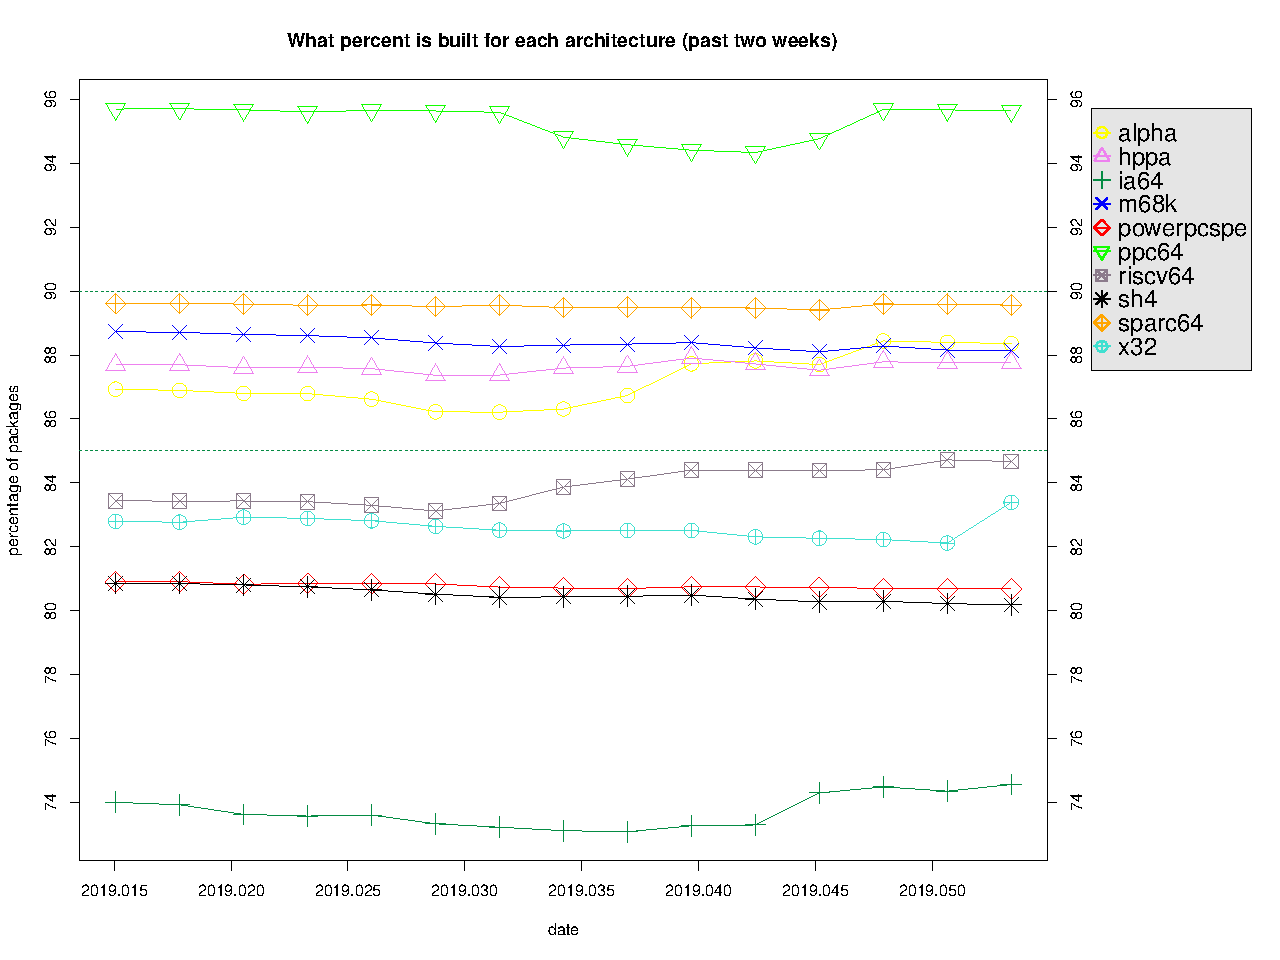
\includegraphics[width=1\textwidth]{figures/graph-ports-week-big}
    \caption{Debian-ports architectures
        \cite["Two weeks report"]{debian_debian-ports_architectures} accessed on 2019-01-22}
    \label{fig:graph-ports-week-big}
\end{figure}
The progress can be seen in figure
\ref{fig:graph-ports-week-big}. Until today
(2019-01-22) already 84 percent of all
Debian source packages have been ported.
About 9000 of the 13000 packages that are architecture
dependent are already building fine, which is already
higher than the number of packages that are available
for the Intel Itanium architecture 
(ia64 in figure \ref{fig:graph-ports-week-big})
\cite[min.~5:35]{youtube_linux_kernel_current_status}.

\subsubsection{Genode}
Genode is a free operating system framework that can run
on many kernels:
\begin{itemize}
    \item{Linux kernel}
    \item{NOVA microhypervisor}
    \item{Base hardware implementation}
    \item{Mue separation kernel}
    \item{seL4 microkernel}
    \item{Fiasco.OC microkernel}
    \item{L4ka::Pistachio microkernel}
    \item{OKL4 microkernel}
\end{itemize}
\cite{genode_platforms} \newline
For RISC-V the base hardware implementation of Genode
has been ported.
It should also be possible to use the Linux kernel as
it is also being ported to RISC-V.
The Genode team described the porting of Genode
as a "rough ride" \cite{genode_risc-v_port}.
They encountered multiple issues with the RISC-V toolchain
being out of sync with the specification and additional
problems with newer pushed versions of GCC that they could
not use for their project \cite{genode_risc-v_port}.
It seems that in the early stages
of development when Genode started working on the port
for RISC-V (2015), the ISA was under heavy development.
The most recent presentation of "RISC-V State of the
Union" at the Santa Clara Convention Center by Krste Asanovic
\cite{risc-v_state_of_the_union_dec_2018}
suggests that in 2019 this situation will be better,
as the RV32 and RV64 bases and the General extension
have been frozen.

\section{Implementations}
There exist many implementations ranging from minimal educational
implementations to larger scalable multi-core ones, 
even Western Digital recently released their new SweRV kernel
which will be used in SSD in the future \cite{anandtech_wd_swerv_ssds}.
This section will mainly talk about the implementations from
the University of Berkeley because they cover the complete spectrum
from simple microcontrollers to more advanced out-of-order
processors.
The University of Berkeley currently develops three different
implementations of the RISC-V ISA.
\begin{itemize}
    \item Sodor (Collection of simple educational processors)
    \item Rocket (In-Order processor)
    \item Berkeley Out-of-Order Machine (Out-of-order Processor)
\end{itemize}
All of the projects use the Constructing Hardware in a Scala
Embedded Language (Chisel) as a programming language. As the
name indicates, this language is implemented in Scala.

\subsection{Scala}
Scala is a general-purpose programming language with a strong
object-oriented static type system which it inherited from Java
\cite{alexander_scala_cookbook}.
The language uses the Actor model to simplify concurrent
programming and make use of many threads, hence the name
Scala from scalable.
\begin{tcolorbox}[colback=SkyBlue, box align=top]
\textbf{Actor model} \cite{hewitt_actor_model}: The actor model is a model
that enables concurrent computing. In the model, one process
is an isolated actor. An actor can:
\begin{itemize}
    \item Make local decisions and computations
    \item Create more actors
    \item Send messages to other actors
\end{itemize}
One actor can not directly modify the state of another actor.
He can only send them messages.
\end{tcolorbox}
\mbox{}\\
Scala builds on Java and thus can use the wide ranges of Java libraries.
It also runs on the JVM.
Programming in Scala is expressive and might sometimes give a feeling
of functional programming.
A simple print loop, for example, looks like this
\begin{lstlisting}[language=scala, frame=single]
    for (i <- Array(1,2,3)) println(i)
\end{lstlisting}
Modification of the Array is achieved via the yield \textit{command}
or the \textit{map} command
\begin{lstlisting}[language=scala, frame=single]
    for (i <- Array(1,2,3)) yield i * 2
    -> Array(2,4,6)
    
    for (i <- Array(1,2,3)).map(_ * 2)
    -> Array(2,4,6)
\end{lstlisting}
Examples taken from the brilliant Scala Cookbook
\cite[p.~xiv-xv]{alexander_scala_cookbook}. \newline
Other functions like \textit{.filter} are also available.
Scalas first version 1 was released in 2003 and has since been
developed to version 2.12. Many companies use Scala to power
their website, including Twitter, Netflix, Tumblr, LinkedIn,
Foursquare, and many more \cite[p.~xiii]{alexander_scala_cookbook}.
The language is best used with the Simple Build Tool (sbt)
that can automate the build process. It builds on the folder
structure of Maven and thus can use existing Maven packages.

\subsection{Chisel}
With Chisel it is possible to develop an FPGA design without
writing one line of Verilog or VHDL but, in the end, have a synthesized
design in one of these languages. Chisel can transform
the code into Verilog, VHDL, and C++.
Until now the development focus was the Verilog ouput
\footnote{https://stackoverflow.com/questions/49587973/converting-chisel-to-vhdl-and-systemc}.
The language supports three primitive types:
\begin{itemize}
    \item UInt (Unsigned integer)
    \item SInt (Signed integer)
    \item Bool (Boolean value)
\end{itemize}
which can be declared as variables like this:
\begin{lstlisting}[language=scala, frame=single]
    val number = UInt(42)
    val answer = Bool(true)
\end{lstlisting}
A user can expand this limited types with so-called bundles:
\begin{lstlisting}[language=scala, frame=single]
    class MyFloat extends Bundle {
        val sign = Bool()
        val exponent = UInt(width=8)
        val significand = UInt(width=23)
    }
\end{lstlisting}
Example taken from \cite[p.~11]{risc-v_chisel} \newline
The class in the example above extends itself from the base
class bundle and defines three values. Two of the variables
define an unsigned integer of the size 8 and 23.
If a new data type is created, new included functions can
also be defined.
Below a implementation of a 2D-vector can be seen:
\begin{lstlisting}[language=scala, frame=single]
    class 2D-Vector(val first: SInt, val second: SInt) extends Bundle {
        def + (b : 2D-Vector): 2D-Vector =
            new 2D-Vector(first + b.first, second + b.second)
        def - (b : 2D-Vector): 2D-Vector =
            new 2D-Vector(first - b.first, second - b.second)
        ...
    }
    
    val x = new 2D-Vector(SInt(20), SInt(32))
    val y = new 2D-Vector(SInt(10), SInt(45))
    val result = x - y
    -> 2D-Vector(10, -13)
\end{lstlisting}
The class above defines two operations, namely addition \textit{+} and
subtraction \textit{-}. The definitions are executed below the definition.
For more complex procedures a module can be defined:
\begin{lstlisting}[language=scala, frame=single]
    class Stack(val depth: Int) extends Module {
        val io = new Bundle {
            val push = Bool(INPUT)
            val pop = Bool(INPUT)
            val en = Bool(INPUT)
            val dataIn = UInt(INPUT, 32)
            val dataOut = UInt(OUTPUT, 32)
        }
        val stack_mem = Mem(UInt(width = 32), depth)
        val sp = Reg(init = UInt(0, width = log2Up(depth+1)))
        val dataOut = Reg(init = UInt(0, width = 32))
        when (io.en) {
            when(io.push && (sp < UInt(depth))) {
                stack_mem(sp) := io.dataIn
                sp := sp + UInt(1)
            } .elsewhen(io.pop && (sp > UInt(0))) {
                sp := sp - UInt(1)
            }
            when (sp > UInt(0)) {
                dataOut := stack_mem(sp - UInt(1))
            }
        }
    
        io.dataOut := dataOut
    }
\end{lstlisting}
This is an implementation of a stack with a data element width
of 32 bit. At first, the \textit{io} variable with definitions of output
and input wires are defined, then the stack memory with a
predefined size (\textit{depth}) is declared.
At last we define the stack pointer (\textit{sp}) with a
width of $\log_{2} n$ (so its values can address 
the complete \textit{stack\_mem}) and the data output (\textit{dataOut})
as register variables (\textit{Reg()}, variables 
retain values till they are changed).
After the definition of variables the stack logic on
the enable signal (\textit{io.en}) is defined.
This stack implementation can also be tested directly in Chisel.
\begin{lstlisting}[language=scala, frame=single]
    class StackTests(c: Stack) extends Tester(c) {
        var nxtDataOut = 0
        val stack = new ScalaStack[Int]()
        for (t <- 0 until 16) {
            val enable = rnd.nextInt(2)
            val push = rnd.nextInt(2)
            val pop = rnd.nextInt(2)
            val dataIn = rnd.nextInt(256)
            val dataOut = nxtDataOut
            if (enable == 1) {
                if (stack.length > 0)
                    nxtDataOut = stack.top
                if (push == 1 && stack.length < c.depth) {
                    stack.push(dataIn)
                } else if (pop == 1 && stack.length > 0) {
                    stack.pop()
                }
            }
            poke(c.io.pop, pop)
            poke(c.io.push, push)
            poke(c.io.en, enable)
            poke(c.io.dataIn, dataIn)
            step(1)
            expect(c.io.dataOut, dataOut)
        }
    }
\end{lstlisting}
Example taken from \cite[p.~45]{risc-v_chisel}\newline
A significant feature of Chisel is the great configurability.
More on that in subsection \ref{rocket-chip}.
\subsection{Sodor}
Sodor is a group of educational implementations of the RISC-V
ISA from the university Berkeley. The five implementations
employ the basic RV32I variant of the base ISA and support
no virtual memory (to keep them as simple as possible).
The cores can be differentiated by the count of
stages they use:
\begin{itemize}
    \item 1-stage (essentially an ISA simulator)
    \item 2-stage (demonstrates pipelining in Chisel)
    \item 3-stage (uses sequential memory)
    \item 5-stage (can toggle between fully bypassed or fully interlocked)
    \item "bus"-based micro-coded implementation
\end{itemize}
All Sodor core use Chisel as a programming language
and can be downloaded on the GitHub page
\cite{github_risc-sodor}.
The 3-stage Sodor implementation was renamed in 2015 to Z-scale
\cite{risc-v_z-scale} and was developed further 
as a smaller alternative to the Rocket Chip SoC generator.
Since 2017-03-30, the repository has received no update,
and the project is deprecated \cite{github_z-scale}.
According to an user on StackOverflow \cite{stackoverflow_zscale},
a similar result to a Z-scale core can be generated by
running the Rocket Chip Generator with the "TinyConfig" configuration.
\begin{lstlisting}[language=bash, frame=single]
    cd vsim
    make verilog CONFIG=TinyConfig
\end{lstlisting}

\subsection{Rocket Chip}\label{rocket-chip}
Rocket Chip is a highly flexible open source generator
written in Chisel and maintained by SiFive and the University
of Berkeley. It generates so-called tiles that
each contains one Rocket core, private caches and optional
ROCC accelerators that
surround the core. To ensure communication a fitting
Uncore module with coherence agents shared caches,
DMA engines and memory controllers are added, and
everything is "glued" together
\cite{risc-v_workshop_jan2015}.

\subsubsection{Tiles}
\begin{figure}
    \centering
    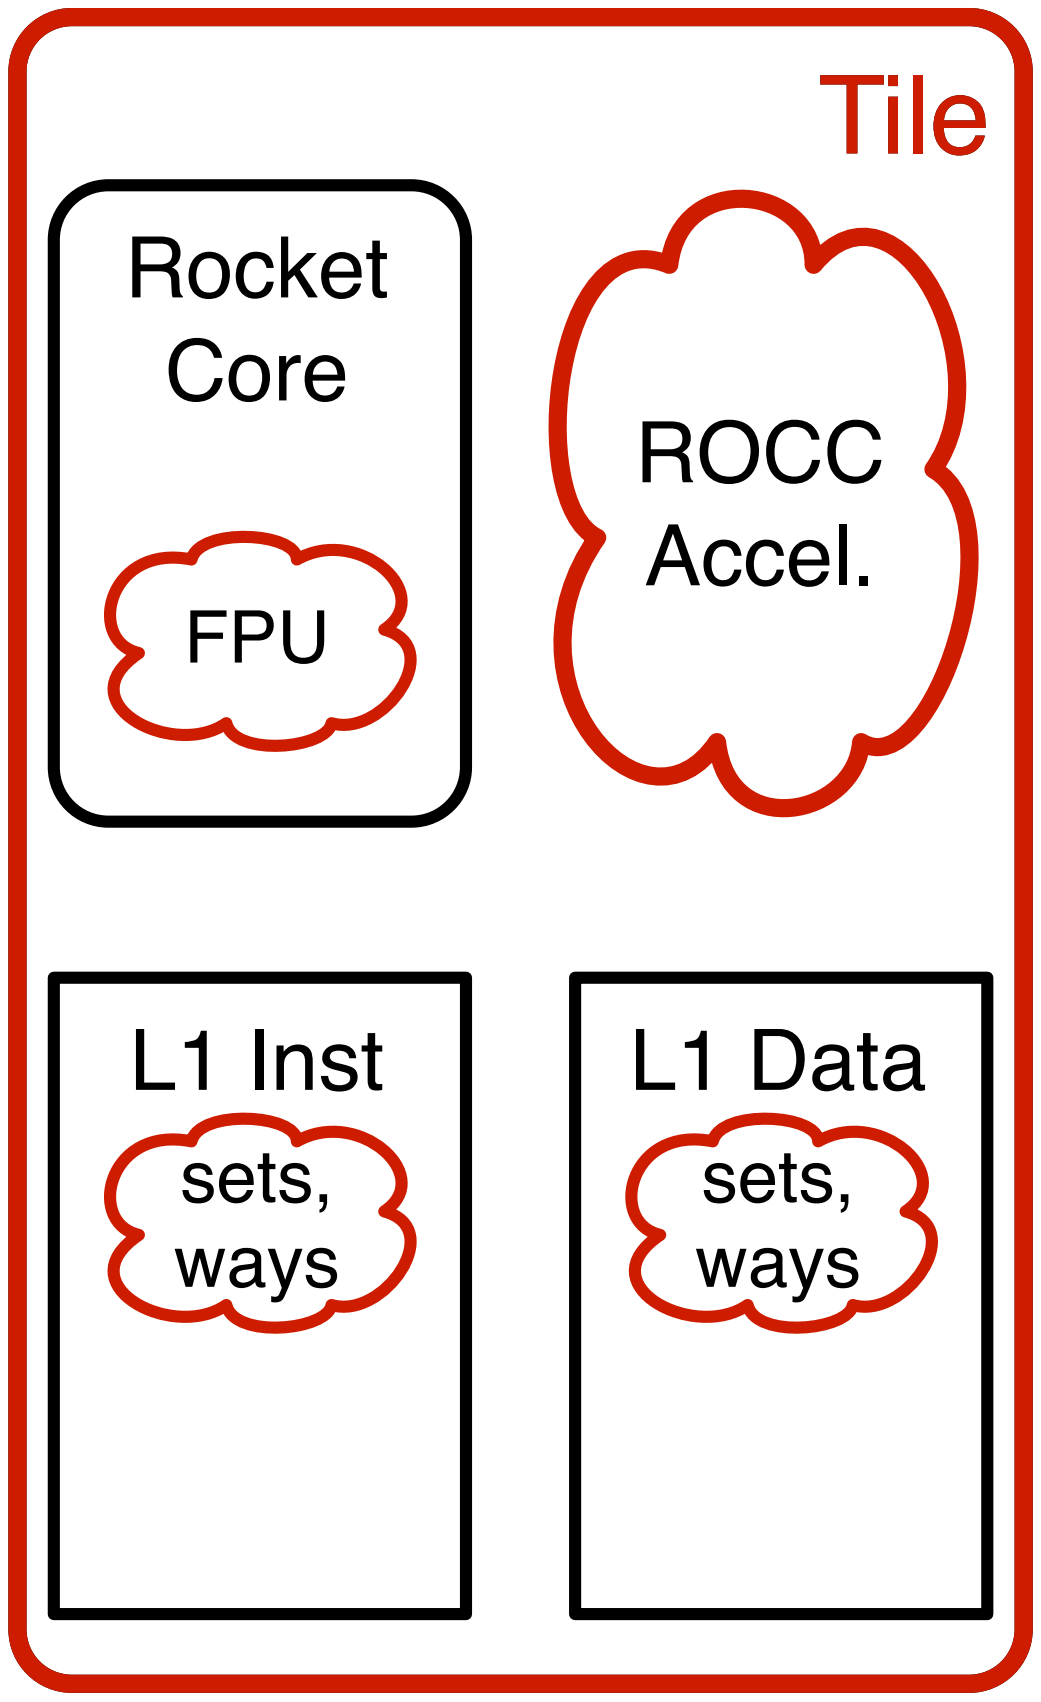
\includegraphics[width=0.4\textwidth]{figures/rocket_chip_tile}
    \caption{A Tile with a Rocket core inside \cite[p.~3]{risc-v_workshop_jan2015}}
    \label{fig:rocket_chip_tile}
\end{figure}
A tile forms one minimal computing complex in a
Rocket Chip. A quad-core design, for example,
will contain four tiles.
Every tile will have their own private instruction
and data L1 caches, as can be seen in figure
\ref{fig:rocket_chip_tile}. The variables \textit{sets} and
\textit{ways} in the cloud in the figure define how
large the cache is and how the connection is
handled. A typical configuration would be:
\begin{lstlisting}[language=scala, frame=single]
    case CacheName("L1D") => CacheConfig(
    nSets = 64,
    nWays = 4,
    rowBits = site(L1toL2Config).beatBytes*8,
    nTLBEntries = 8,
    cacheIdBits = 0,
    splitMetadata = false)
\end{lstlisting}
To speed up certain computation tasks an
FPU can be added directly in the Rocket core,
or a ROCC accelerator is included in the tile.
A nice example of such an accelerator is shown
by the Celerity \cite{celerity_manycore}, \cite{opencelerity_page}
that was created from 20 graduate
students in a combined effort of the University of
Michigan, UC San Diego, the University of 
Washington and the Cornell University.
Their design houses 511 RISC-V cores with
different levels of complexity.
5 Linux capable, general-purpose
RV64G Rocket cores control the
system and execute the operating system.
Next to them, 496 RV32IM Rocket cores are packaged
in a mesh tiled array together to form the manycore
tier. Ten additional low voltage cores are
placed next to the manycore package.
To accelerate the computation further, the
Accelerating Binarized Neural Networks are added
as a third specialization tier, which can communicate
with the manycore tier and the general-purpose tier.
The construction can be seen in
\ref{fig:celerity_design}.
\begin{figure}
    \centering
    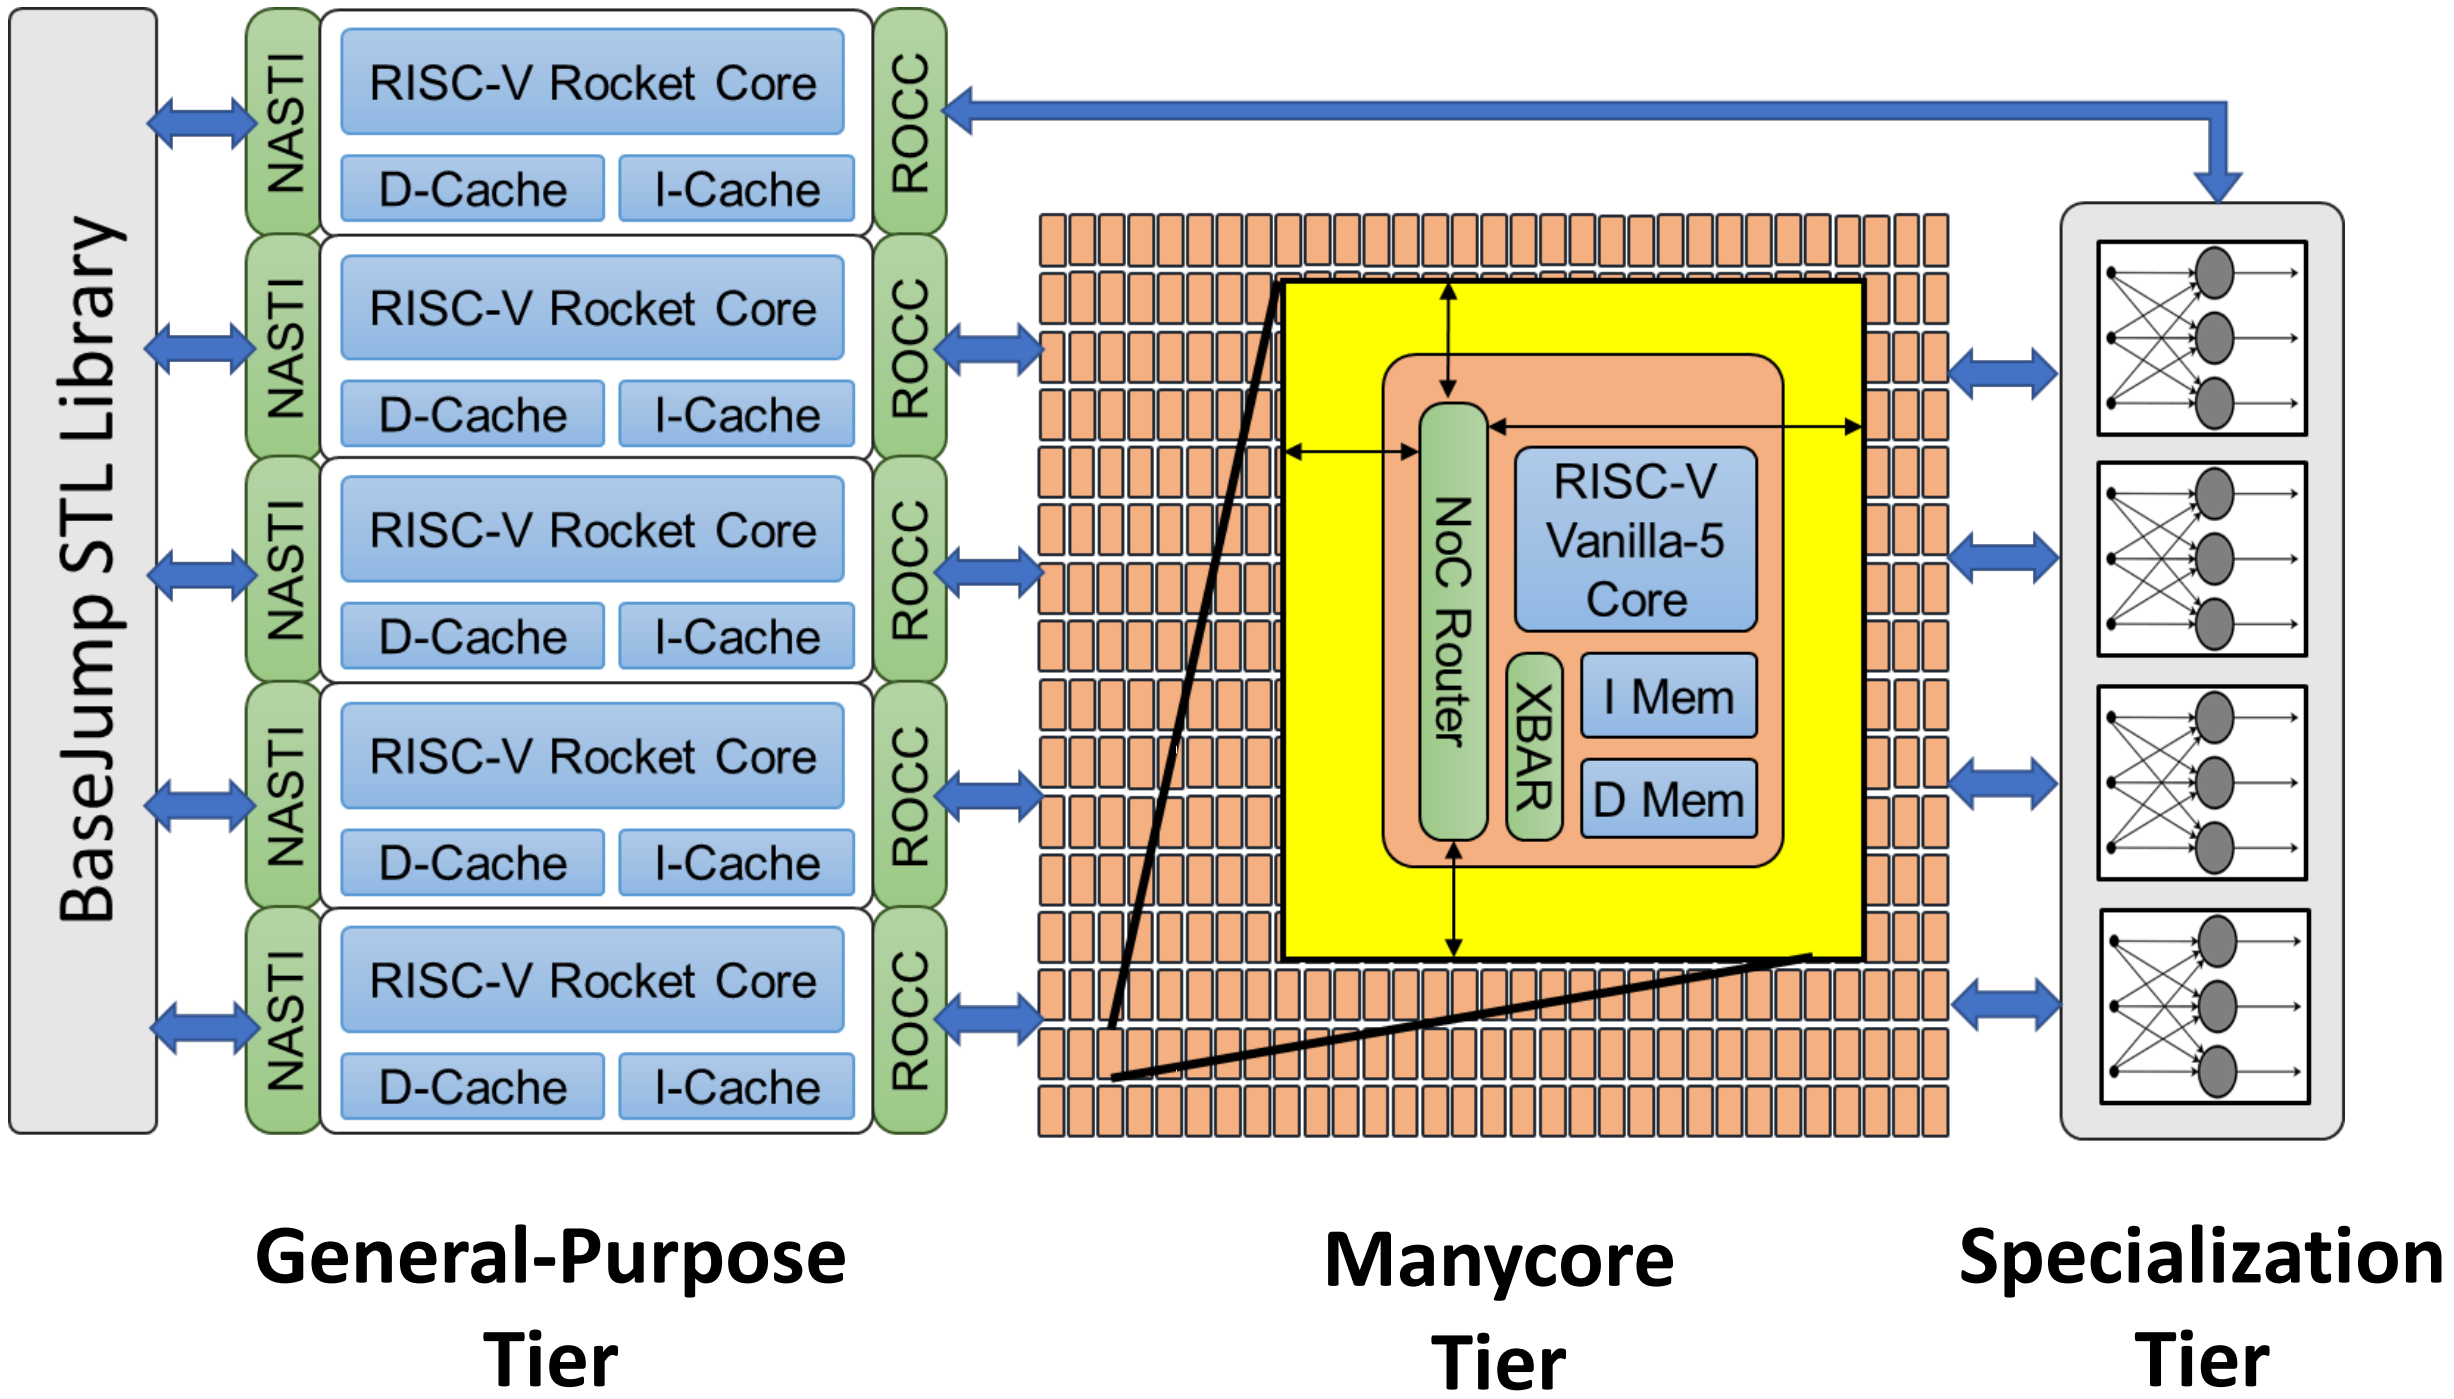
\includegraphics[width=0.9\textwidth]{figures/celerity_design}
    \caption{Overview of the Celerity architecture \cite{opencelerity_page}}
    \label{fig:celerity_design}
\end{figure}
The ROCC interface makes it possible for developers
to easily include accelerators in a Rocket Chip architecture.

\subsubsection{Interconnects}
As it can be seen in figure \ref{fig:celerity_design}
general-purpose tier tiles are connected with NASTI
interfaces to the rest of the hardware on the system
(memory, I/O, ...). \textbf{N}ot \textbf{A}
\textbf{ST}andard \textbf{I}nterface
(NASTI, pronounced nasty) is the
implementation of the University of Berkeley of the
AXI-standard from Xilinx. It is necessary to
use this interface if one wants to develop designs
on Xilinx FPGA hardware, but it is not the only
interface available:
\begin{itemize}
    \item TileLink
    \item NASTI (pronounced nasty) 
    \item HASTI (pronounced hasty)
    \item POCI (pronounced pokey)
\end{itemize}
TileLink will be explained in the next subsection.
Highly Advanced System Transport Interface (HASTI) is the
implementation of the University of Berkeley for the
AHB-Lite standard from ARM.
A similar implementation is the
Peripheral Oriented Connection Interface (POCI)
which is the implementation of the AHB standard,
from ARM.
The last two standards are used for the communication
with ARM cores that are bound to the AHB/AHB-lite
standard \cite{risc-v_z-scale}.

\subsubsection{TileLink}\label{chapter:tilelink}
When the development of Rocket-Chip started the
developers were confronted with a problem.
They needed a bus system that fulfills the
following requirements:
\begin{itemize}
    \item Open standard
    \item Easy to implement
    \item Cache-coherent block motion (Moving cache blocks around)
    \item Multiple cache layers
    \item Reusable on- and off-chip
    \item High performance
\end{itemize}
They considered AHB, Wishbone, AXI4, ACE and CHI as
standards for the bus system, but none of them
fulfilled all requirements that were previously set.
Additionally, if they would rely on a standard from a
competitor (ARM: AHB, CHI, ACE; Xilinx: AXI4, 
Opencores(Silicore): Wishbone), they
could change the standard or hold back documents to
slow down the development.
So the team decided to reuse an academic already existing
bus protocol called TileLink and develop it further.
TileLink is a Master-Slave protocol, with 5 priorities (A,B,C,D,E).
Messages can be sent out-of-order with optional
ordering. It was designed to be composable and
deadlock free.
TileLink comes in three versions that build on each other, shown
in table \ref{tab:tilelink_levels}.
\begin{table}
    \caption{Comparison of TileLink conformance levels
        \cite[p.~10]{risc-v_tilelink}}
    \centering
    \label{tab:tilelink_levels}
    \begin{tabular}{|l|l|l|l|}
    \hline
         & TL-UL & TL-UH & TL-C \\ \hline
        Read/Write operations & x & x & x \\ \hline
        Multibeat Messages &  & x & x \\ \hline
        Atomic operations &  & x & x \\ \hline
        Hint (prefetch) operations &  & x & x \\ \hline
        Cache block transfers &  &  & x \\ \hline
        Priorities B+C+E &  &  & x \\ \hline
    \end{tabular}
\end{table}
The written-out names of the conformance levels are:
\begin{itemize}
    \item TL-UL: TileLink uncached lightweight
    \item TL-UH: TileLink uncached heavyweight
    \item TL-C: TileLink cached
\end{itemize}
It is possible to use multiple levels on the same chip for
different components like it is shown in the schematic of the
SiFive FU500 design in figure \ref{fig:sifive_fu500}.
\begin{figure}
    \centering
    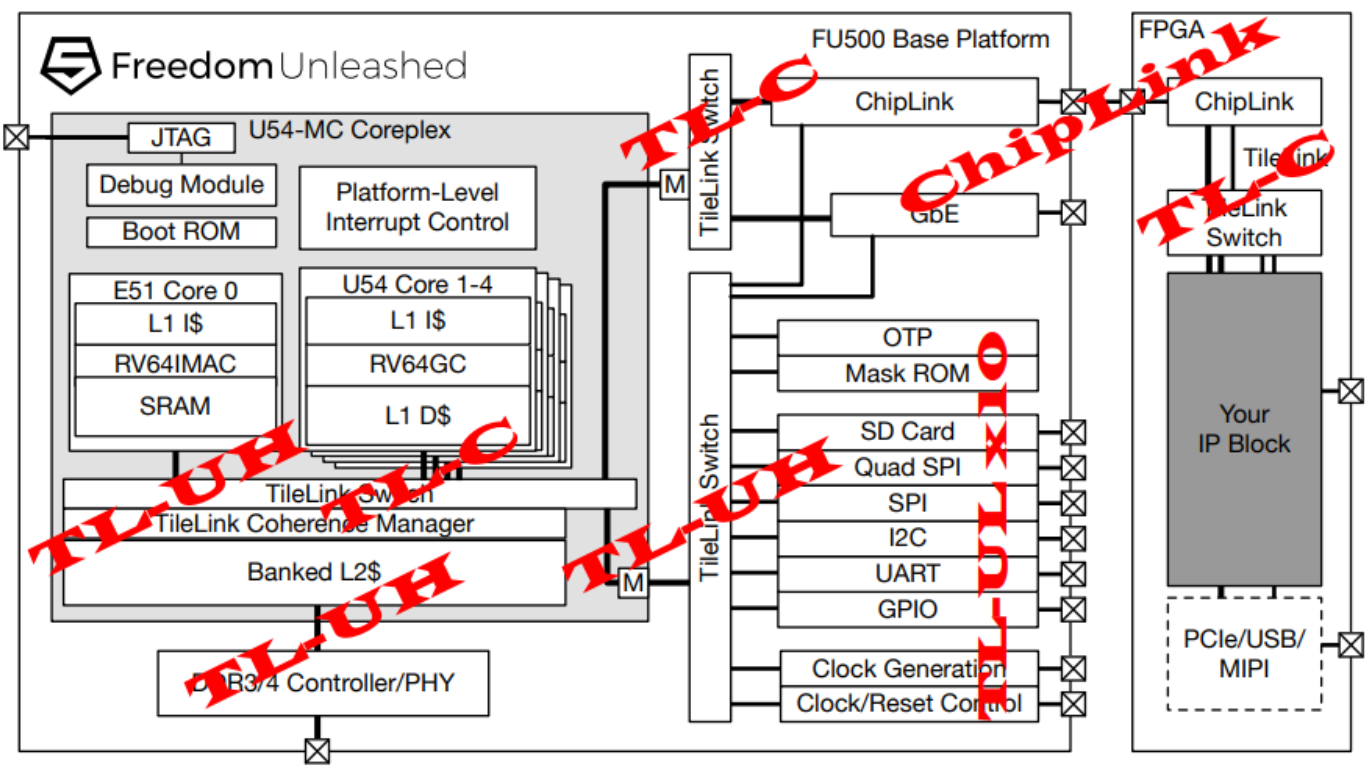
\includegraphics[width=0.9\textwidth]{figures/sifive_fu500}
    \caption{Schematic of SiFive FU500
        \cite[p.~25]{risc-v_tilelink}}
    \label{fig:sifive_fu500}
\end{figure}

\subsection{Berkeley Out-of-Order Machine (BOOM)}
Berkeley Out-of-Order Machine (BOOM) builds on top
of the Rocket Chip SoC ecosystem and expands
it with out-of-order execution. BOOM consists of
about 16 thousand lines of Chisel code and is,
as the Rocket Chip generator, an open-source chip generator.
BOOMv1.0 was first released on 14. July 2017 and
replaced by BOOMv2 on 16. August 2017.
Since then the v2 version has matured to version
2.2.0. The use of out-of-order execution, should in
the future, speed up the computations of the processor.


\section{Comparing implementations}
As the interest in RISC-V grows, so does the count of implementations
of the RISC-V ISA in software and hardware. In the following diagram
mainly RISC-V implementations are compared against ARMs solutions and one
custom soft microprocessor solution from the manufacturer Xilinx.
Processors need to adapt to the problems they need to solve, and
as there is an uncountable amount of problems, a 
comparison between the corresponding processors could be
infinitely large as well.
The following comparison groups the processors by their included
features to get a better overview:

\begin{enumerate}
    \item No FPU, No MMU: Very basic microcontroller, mostly used
    in applications where power is very restricted.
    \item FPU, No MMU: Limited processor for embedded systems that
    need a hardware acceleration but often are focused on a limited
    set of tasks.
    \item FPU, No MMU but PMP: Larger processor for embedded systems
    that runs mostly more than one process and thus needs a certain
    level of delimitation between processes.
    \item FPU, MMU: Processors capable of running a general purpose
    operating system like Linux that uses virtual address spaces.
\end{enumerate}
Abbreviations used:\\
FPU = Floating Point Unit, MMU = Memory Management Unit, 
PMP = Physical Memory Protection


\begin{table}[htpb]
  \caption[Comparison of chip implementations]{Comparison of chip implementations}\label{tab:comparison_implementations}
  \centering
    \begin{tabular}{| l | l | l | l | l |}
        \hline
        % header
        \begin{tabular}{@{}l@{}}
             Implementation
        \end{tabular} &
        \begin{tabular}{@{}l@{}}
            No FPU  \\ No MMU  
        \end{tabular} &
        \begin{tabular}{@{}l@{}}
            FPU  \\ No MMU   
        \end{tabular} &
        \begin{tabular}{@{}l@{}}
            FPU  \\ No MMU but PMP 
        \end{tabular} &
        \begin{tabular}{@{}l@{}}
            FPU  \\ MMU
        \end{tabular} \\ \hline
        %entries
        \begin{tabular}{@{}l@{}}
             ARM \\ M0, M0+, M1, M3
        \end{tabular} & 
        X & & & \\ \hline
        
        \begin{tabular}{@{}l@{}}
             ARM \\ M4, M7, M33, M35P
        \end{tabular} & 
        X & (optional) & &  \\ \hline
        
        \begin{tabular}{@{}l@{}}
             ARM \\ R-Series
        \end{tabular} & 
        X & (optional) & (optional) &  \\ \hline
        
        \begin{tabular}{@{}l@{}}
             ARM \\ A-Series
        \end{tabular} & 
         & & & X  \\ \hline
        
        \begin{tabular}{@{}l@{}}
             SiFive \\ E-Series
        \end{tabular} & 
        X & (optional) & &  \\ \hline
        
        \begin{tabular}{@{}l@{}}
             SiFive \\ S-Series
        \end{tabular} & 
         & & X &  \\ \hline
        
         \begin{tabular}{@{}l@{}}
             SiFive \\ U-Series
        \end{tabular} & 
         & & & X  \\ \hline
        
        \begin{tabular}{@{}l@{}}
             Pulp Platform \\ Micro-Riscy, Zero-Riscy
        \end{tabular} & 
        X & & &  \\ \hline
        
        \begin{tabular}{@{}l@{}}
             Pulp Platform \\ RI5CY
        \end{tabular} & 
         & X & (optional) & \\ \hline
        
        \begin{tabular}{@{}l@{}}
             Pulp Platform \\ Ariane
        \end{tabular} & 
         & & & X  \\ \hline
        
        \begin{tabular}{@{}l@{}}
             Greenwaves \\ GAP8
        \end{tabular} & 
        X & & &  \\ \hline
        
        \begin{tabular}{@{}l@{}}
             Kendryte \\ K210
        \end{tabular} & 
         & & & X  \\ \hline
        
        \begin{tabular}{@{}l@{}}
             Xilinx \\ MicroBlaze (no RISC-V)
        \end{tabular} & 
         & & & X  \\ \hline
    \end{tabular}
\end{table}

\section{Competition}
As the market for processors architecture has grown
over the years, RISC-V is faced with many competitors.
Some of these are described in the following subsections.

\subsection{ARM}
ARM is one of the largest competitors of RISC-V. Many
smaller ARM chips are built into embedded systems, which
can be replaced by a RISC-V processor.
ARM is away of its new competitor and launched a marketing campaign
website against RISC-V in July 2018 which promoted the
disadvantages of the RISC-V architecture.
The campaign website has since been taken down after
internal and external protests \cite{theregister_arm_campaign_risc-v}.
The website has also been removed from \textit{web.archive.org}
\footnote{\url{https://web.archive.org/web/20180708231736/https://riscv-basics.com/}},
were a cached version was still accessible shortly after the
reports were published.

\subsection{MIPS}
MIPS is like RISC-V a RISC architecture and has been acquired in
June 2018 by the AI Startup Wave Computing
\cite{top500_mips_acquired}. Wave Computing announced that in
the first quarter of 2019 they would open up the ISA for other developers and further
development will happen under the new MIPS Open initiative
\cite{wavecomputing_mips_open}.
In contrast to RISC-V Wave computing still requires a sign up
to access the ISA and extensions to it.
The MIPS ISA could be a significant competitor to RISC-V,
as it has already been taped out many times, also runs
the Linux kernel and is now free to use.

\subsection{x86 and other high-performance architectures}
RISC-V currently has not yet achieved a tap-out of
high performance. The Linux capable SiFive HiFive Unleashed board with
its four cores at 1.5GHz 
\cite{risc-v_sifive_hifive} is already a step in the right
direction but far from a desktop pc grade chip.
SiFive also has announced the U74-MC processor with up to eight cores,
which is said to perform equally to an ARM-A55 (that is used in many
mobile phones) \cite{linuxgizmos_sifive_u74}.
RISC-V will be a competitor for high-performance
chips, but the implementation of this new version are
not ready yet.